\documentclass{article}

\usepackage[left=2cm,right=2cm,top=2cm,bottom=2cm]{geometry} 

\usepackage[utf8]{inputenc}   % otra alternativa para los caracteres acentuados y la "ñ"
\usepackage[           spanish % para poder usar el español
                      ,es-tabla % para los captions de las tablas
                       ]{babel}   
\decimalpoint %para usar el punto decimal en vez de coma para los números con decimales

%\usepackage{beton}
%\usepackage[T1]{fontenc}

\usepackage{parskip}
\usepackage{xcolor}

\usepackage{caption}

\usepackage{enumerate} % paquete para poder personalizar fácilmente la apariencia de las listas enumerativas

\usepackage{graphicx} % figuras
\usepackage{subfigure} % subfiguras

\usepackage{amsfonts}
\usepackage{amsmath}

\usepackage{listings}
\lstset
{ %Formatting for code in appendix
    language=python,
    basicstyle=\footnotesize,
    stepnumber=1,
    showstringspaces=false,
    tabsize=1,
    breaklines=true,
    breakatwhitespace=false,
}

\definecolor{gris}{RGB}{220,220,220}
	
\usepackage{float} % para controlar la situación de los entornos flotantes

\restylefloat{figure}
\restylefloat{table} 
\setlength{\parindent}{0mm}


\usepackage[bookmarks=true,
            bookmarksnumbered=false, % true means bookmarks in 
                                     % left window are numbered
            bookmarksopen=false,     % true means only level 1
                                     % are displayed.
            colorlinks=true,
            allcolors=blue,
            urlcolor=blue]{hyperref}
\definecolor{webblue}{rgb}{0, 0, 0.5}  % less intense blue


\title{\Huge Inteligencia de Negocio: Práctica 2 \\ Visualización y Segmentación\vspace{10mm}}

\author{\huge David Cabezas Berrido \vspace{10mm} \\ 
  \huge Grupo 2: Viernes \vspace{10mm} \\ \huge dxabezas@correo.ugr.es \vspace{10mm}}

\begin{document}
\maketitle
\newpage
\begin{center}
\vspace*{8cm}
{\Huge \textbf{Visualización}}
\end{center}
\newpage
\tableofcontents
\newpage

Sobre los resultados de la práctica 1, realizaremos representaciones
de los scores obtenidos por cada algoritmo para cada
preprocesamiento. No nos centraremos en por qué unos modelos o
preprocesamientos son mejores que otros, ni en detalles de los mismos
(hiperparámetros configurados o por defecto. Eso ya lo hicimos en la
práctica anterior. Nos centraremos cómo podemos interpretar las
visualizaciones para ayudarnos a distinguir qué algoritmo o
procesamiento es más adecuado en cada caso.

\section{Visualización de medidas}
Compararemos los scores de todos los modelos para cada
preprocesamiento y viceversa. Las métricas que representaremos son la
Accuracy y el F1-score.

\subsection{Por procesamiento}

El \textbf{primer procesamiento} consiste en \textbf{eliminar las
  instancias con valores perdidos}.

\begin{figure}[H]
  \centering
  \caption{Desempeño de los algoritmos sobre el preprocesado 1: Eliminación de valores perdidos}
  \label{fig:dropna}
  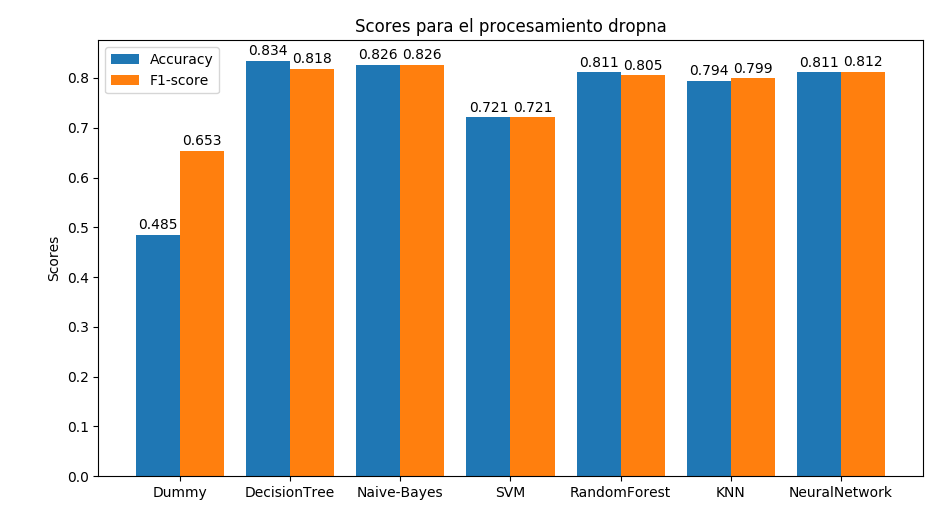
\includegraphics[width=180mm]{figures/visualizacion/dropna}
\end{figure}

La barra azul (Accuracy) representa el desempeño general del modelo,
la proporción de instancias bien clasificadas en validación
cruzada. Mientras que la barra naranja (F1-score) le da una mayor
prioridad a la clasificación de instancias positivas, que tienen mayor
importancia en este problema, puesto que un falso negativo es más
grave que un falso positivo.

Los modelos que más score han obtenido para este preprocesamiento son
el Árbol de Decisión y Naive-Bayes. El Árbol de Decisión tiene
ligeramente mayor Accuracy, mientras que Naive-Bayes tiene más
F1-score, esto significa que Decision Tree clasifica mejor las
instancias negativas que Naive-Bayes, y éste último clasifica mejor
las positivas.

SVM presenta resultados bastante peores al resto de algoritmos
(obviando Dummy).

Generalmente, la Accuracy y la F1-score son similares. La excepción es
Dummy, que clasifica bien todas las positivas pero ninguna negativa.

El \textbf{segundo procesamiento} consiste en \textbf{imputar los
  valores perdidos}, para las variables numéricas usamos la mediana y
para las nominales, la moda.

\begin{figure}[H]
  \centering
  \caption{Desempeño de los algoritmos sobre el preprocesado 2: Imputación de valores perdidos}
  \label{fig:median}
  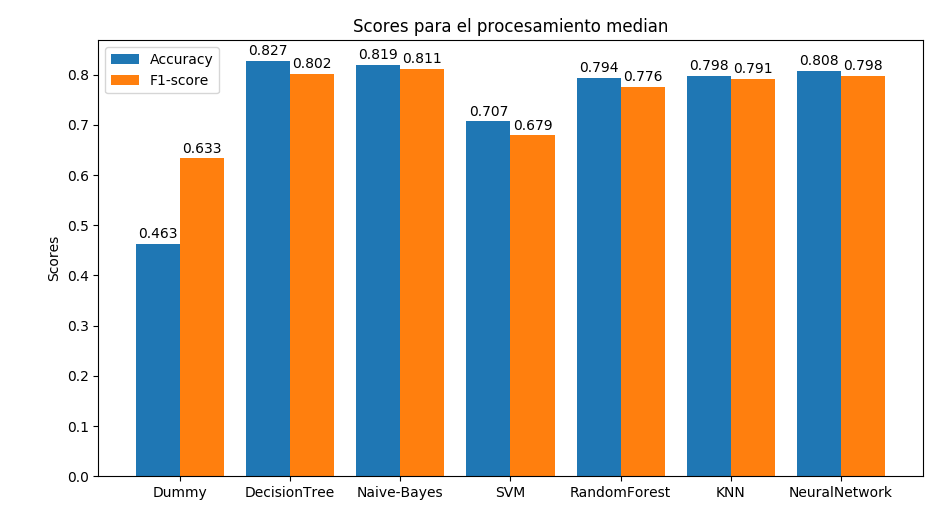
\includegraphics[width=170mm]{figures/visualizacion/median}
\end{figure}

La comparación entre los modelos no ha cambiado mucho, salvo un
descenso en el desempeño de todos los modelos. La gráfica nos ayuda a
observar, comparando las barras azules con las naranjas, que el
descenso ha sido mayor en la F1-score (la barra naranja ahora está más
abajo que la azul en todos los algoritmos salvo Dummy), esto significa
que, en general, ha empeorado la clasificación de instancias
positivas.

El \textbf{tercer procesamiento} consiste en \textbf{simplificar el
  conjunto de atributos}. Concretamente, eliminamos Density y
simplificamos la distribución de BI-Rads para que sólo tome los
valores 4 y 5.

\begin{figure}[H]
  \centering
  \label{fig:features}
  \caption{Desempeño de los algoritmos sobre el preprocesado 3: Eliminación de características innecesarias}
  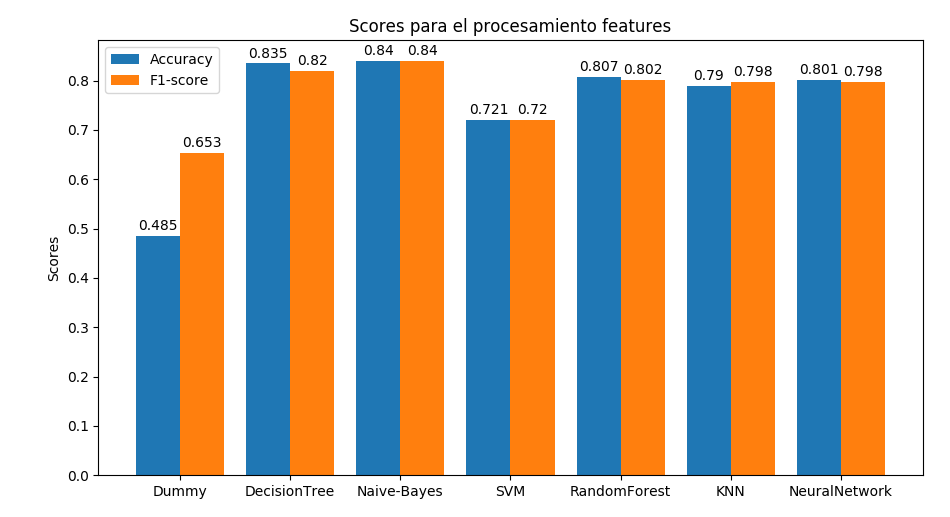
\includegraphics[width=170mm]{figures/visualizacion/features}
\end{figure}

Con este preprocesamiento, observamos que se ha recuperado la
similitud entre los valores de F1-score y Accuracy, puesto que se hizo
sobre los datos del preprocesado 1 y no sobre los del 2. También se ha
producido una mejora general en la mayoría de modelos, sobre todo en
Naive-Bayes por lo que comentamos en la práctica anterior de que
supone los atributos independientes. Sin embargo, la comparación entre
los modelos no cambia demasiado.

El \textbf{cuarto procesamiento} consiste en \textbf{binarizar las
  características nominales}, Shape y Margin. Esto lo hicimos porque
no tenía sentido medir la distancia entre valores de una variable
nominal si los numerábamos con números naturales, y algoritmos que no
tratan bien las variables nominales como KNN y Neural Network podían
verse afectados por esto.

\begin{figure}[H]
  \centering
  \label{fig:binarization}
  \caption{Desempeño de los algoritmos sobre el preprocesado 4: Binarización de características nominales}
  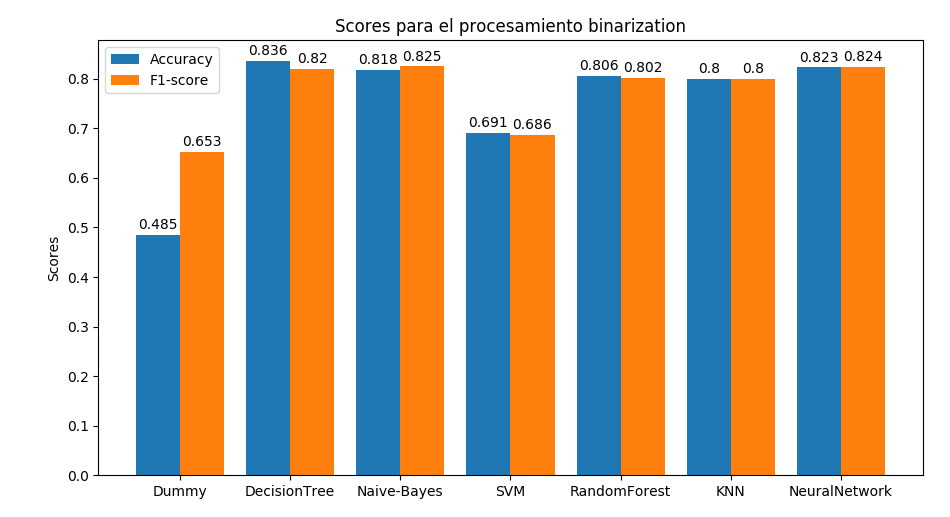
\includegraphics[width=180mm]{figures/visualizacion/binarization}
\end{figure}

Se aprecia un descenso en Naive-Bayes, por haber introducido nuevas
características que no son independientes unas de otras (cuando una
vale 1, el resto de características binarizas asociadas a la misma
variable nominal están forzadas a valer 0). La mejora en KNN es muy
leve, pero sí destaca ahora una subida en la colummna de Neural
Network.

Este procesamiento también perjudica aún más a SVM, aumenta más la
diferencia entre su columna y el resto.

El \textbf{quinto procesamiento} consiste en \textbf{reescalar las
  variables}, para que tengan media 0 y varianza 1. Esto se hizo para
solucionar la importancia exagerada que cobraba la variable Age en
algoritmos como KNN.

\begin{figure}[H]
  \centering
  \label{fig:stdScaler}
  \caption{Desempeño de los algoritmos sobre el preprocesado 5: Estandarizado de los datos}
  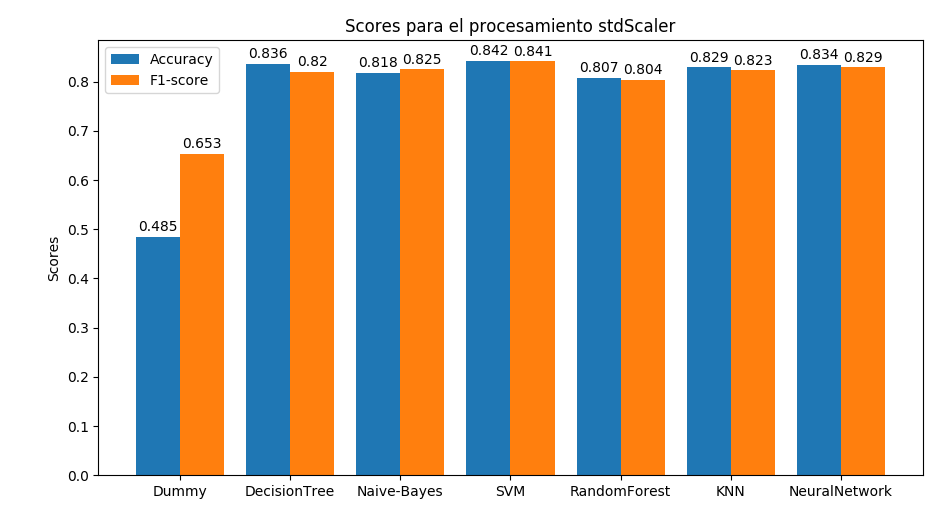
\includegraphics[width=180mm]{figures/visualizacion/stdScaler}
\end{figure}

Lo que más descata en esta gráfica es la importante subida de SVM, su
columna sube hasta acabar ligeramente por encima del resto. También
observamos una subida notable en el desempeño de KNN, cuya barra
adelanta a la de Random Forest.

\subsection{Por modelo}

\begin{figure}[H]
  \centering
  \label{fig:dummy}
  \caption{Desempeño de Dummy para cada preprocesamiento}
  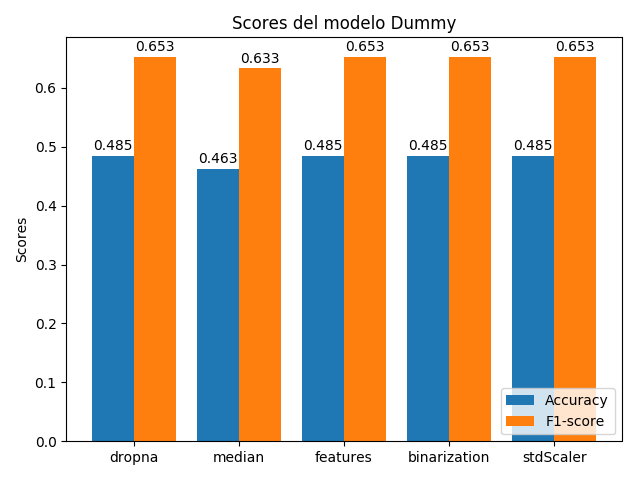
\includegraphics[width=90mm]{figures/visualizacion/dummy}
\end{figure}

No hay mucho que comentar de Dummy, consigue los mismos scores para
todos los preprocesamientos, ya que ignora los datos de entrada y se
limita a predecir siempre maligno. Cambia para el el segundo
preprocesamiento, porque varía el número de instancias, ya que no
eliminamos las instancias con valores perdidos.

\begin{figure}[H]
  \centering
  \label{fig:dt}
  \caption{Desempeño de Decision Tree para cada preprocesamiento}
  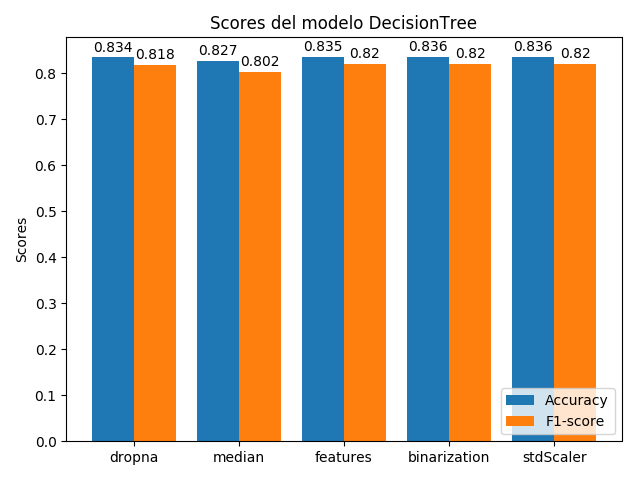
\includegraphics[width=90mm]{figures/visualizacion/decisionTree}
\end{figure}

La eficacia de Decision Tree no se vió afectada apenas por ninguno de
los procesamientos que planteamos. Trabaja con las variables por
separado, por lo que no le afecta el reescalado; trabaja bien con las
variables nominales, por lo que no se ve beneficiado de la
binarización de las mismas. Sí que observamos que este modelo
acostumbra a clasificar mejor las instancias negativas, ya que su
desempeño general (barra azul) está por encima de su F1-score (barra
naranja), que da mayor importancia a los ejemplos positivos.

\begin{figure}[H]
  \centering
  \label{fig:nb}
  \caption{Desempeño de Naive-Bayes para cada preprocesamiento}
  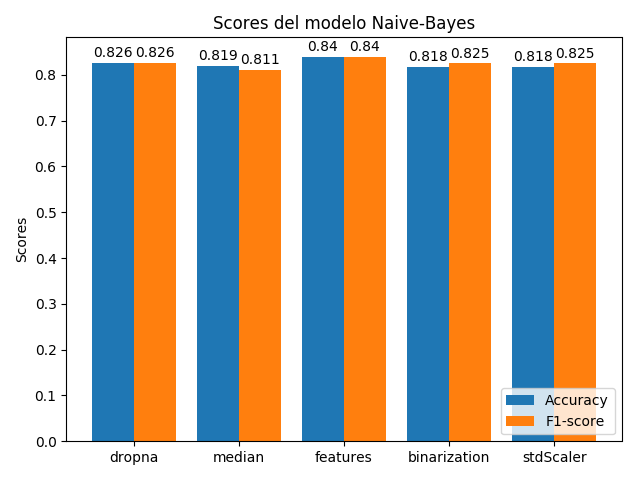
\includegraphics[width=90mm]{figures/visualizacion/gaussianNB}
\end{figure}

Sobre este modelo percibimos que funciona mejor tras la simplificación
del conjunto de características, pero empeora al introducir
características nuevas que no son independientes cuando binarizamos
las características nominales. Sobre algunos preprocesamientos ha
tenido similar desempeño al clasificar instancias positivas y
negativas (las barras azul y naranja están a la misma altura). Al
igual que el resto de modelos, al imputar los valores perdidos pierde
bastante efectividad sobre los ejemplos positivos (la barra naranja
está más abajo que la azul). Al introducir las características
dependientes en la binarización de variables nominales, decrece su
eficacia sobre todo para los ejemplos negativos (la barra naranja no
decrece tanto como la azul), y tampoco se ve afectado por el
reescalado de los datos.

\begin{figure}[H]
  \centering
  \caption{Desempeño de SVM para cada preprocesamiento}
  \label{fig:svm}
  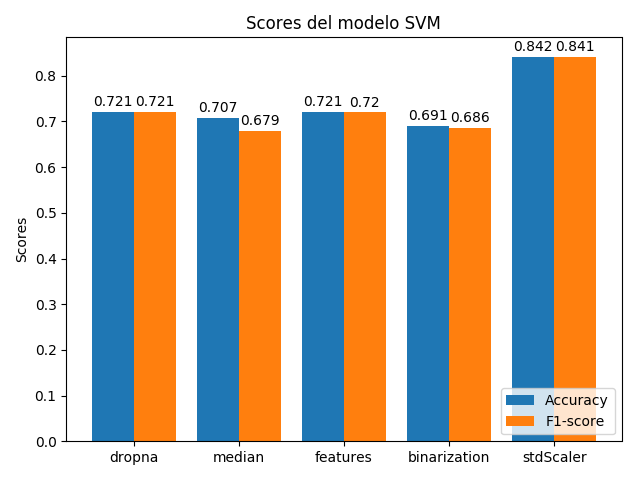
\includegraphics[width=90mm]{figures/visualizacion/svm}
\end{figure}

SVM presenta un desempeño bastante pobre hasta llegar al reescalado de
las variables, cuando se convierte en el modelo que más score
consigue. Se ve perjudicado por la binarización de características
nominales y, exceptuando lo que les ocurre a todos los algoritmos con
el segundo preprocesado (imputar valores perdidos), su desempeño es
similar en las características positivas y en las negativas (las
barras azul y naranja están muy igualadas).

\begin{figure}[H]
  \centering
  \caption{Desempeño de Random Forest para cada preprocesamiento}
  \label{fig:rf}
  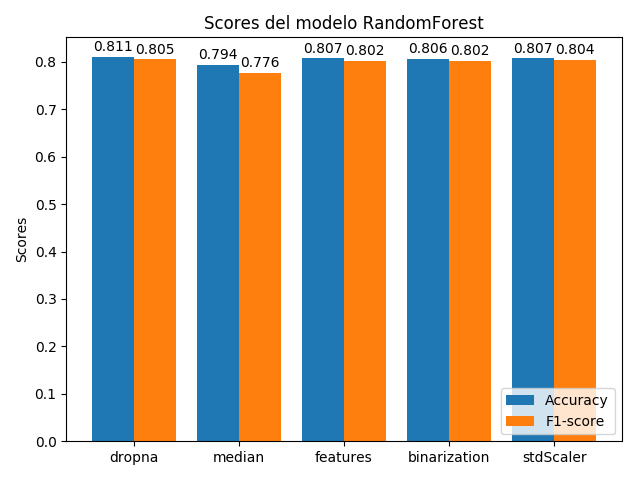
\includegraphics[width=90mm]{figures/visualizacion/randomForest}
\end{figure}

A Random Forest le ocurre lo mismo que a Decision Tree (Random Forest
es un modelo que promedia varios Decision Tree), aunque su desempeño
en general es peor. Hay un poco menos de diferencia entre las barras
azul y naranja, por lo que no empeora tanto al clasificar instancias
positivas.

\begin{figure}[H]
  \centering
  \caption{Desempeño de KNN para cada preprocesamiento}
  \label{fig:knn}
  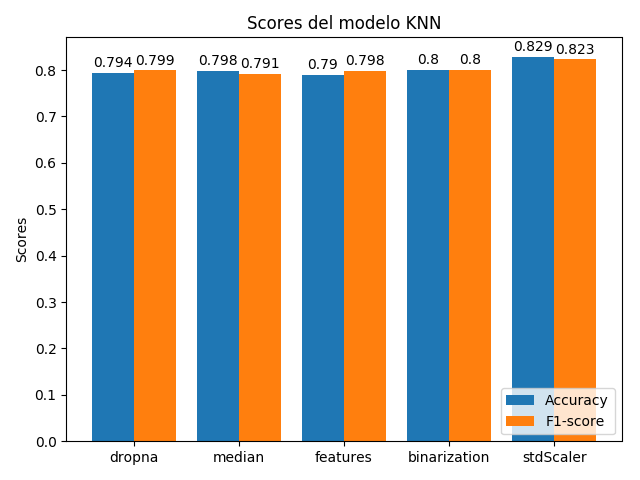
\includegraphics[width=90mm]{figures/visualizacion/knn}
\end{figure}

KNN se ve beneficiado por los dos últimos procesamientos, sobre todo
con el último, el reescalado de las variables. Presenta resultados
similares para todos los procesamientos, en comparación con los otros
modelos, empeora poco con la imputación de valores perdidos. Su
desempeño es similar para todos los preprocesamientos excepto para el
último, donde la mejora es notable.

\begin{figure}[H]
  \centering
  \caption{Desempeño de Neural Network para cada preprocesamiento}
  \label{fig:neuralNetwork}
  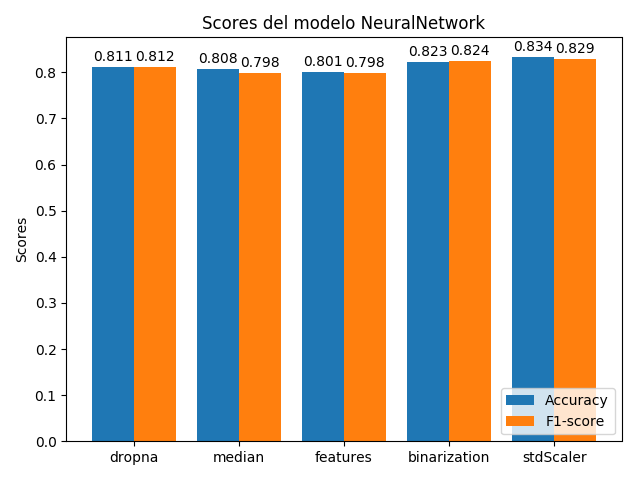
\includegraphics[width=90mm]{figures/visualizacion/neuralNetwork}
\end{figure}

Neural Network se ve perjudicado por la simplificación del conjunto de
características, probablemente porque es un modelo con una alta
complejidad y capacidad explicativa y sea capaz de aprovechas la poca
información que se pierde con esta simplificación. Los preprocesados
de binarización y estandarización le benefician en gran medida. En
general, su eficacia es similar en ejemplos positivos y negativos, las barras azul y naranja están prácticamente a la misma altura.

\section{Gráficas de la curva ROC}

Para cada preprocesamiento, compararemos los modelos representándolos
en el espacio ROC. Los estamos tratando como modelos discretos (sólo
atendemos a la clase que predigan, no la probabilidad que asignen de
pertenencia a cada clase), por lo que no vamos a dibujar sus curva ROC
como es habitual verlas, con forma de codo. Esto podríamos hacerlo con
la función \texttt{roc\_curve} de \texttt{sklearn.metrics}, pero
tenemos que tener claro la interpretación continua que se hace del
modelo para interpretar las curvas. Por ejemplo un árbol de decisión
se puede interpretar como un modelo continuo de la siguiente manera:
si una instancia cae sobre una hoja con $p$ instancias de
entrenamiento de la clase maligno y $q$ de la clase benigno, puede
asignar una probabilidad de $\frac{p}{p+q}$ para la clase maligno y
una de $\frac{q}{p+q}$ para la clase benigno.

En su lugar, cada modelo aparecerá como un punto en el plano,
concretamente en el intervalo $[0,1]\times[0,1]$.

El análisis gráfico por gráfico sería muy repetitivo, por lo que nos
limitaremos a explicar cómo se interpretan estos gráficos. Lo haremos
sobre el primero de ellos.

\begin{figure}[H]
  \centering
  \caption{Algoritmos sobre el preprocesado 1 representados en el espacio ROC}
  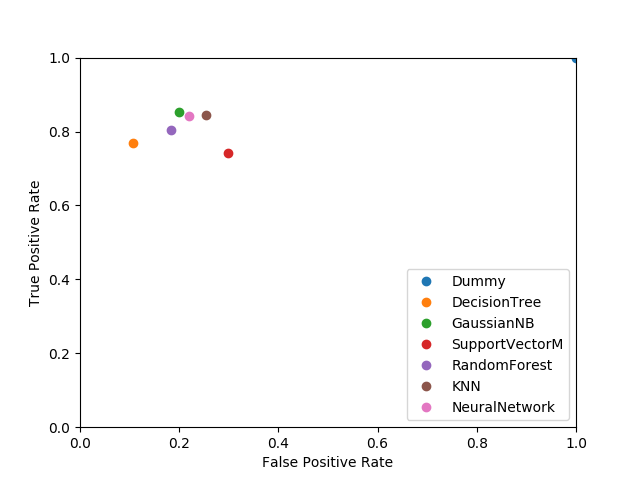
\includegraphics[width=120mm]{figures/visualizacion/roc1}
  \label{fig:roc1}
\end{figure}

En el eje horizontal se representa el FPR, la tasa de falsos positivos
(número de predicciones positivas incorrectas entre el número total de
ejemplos negativos). En el eje vertical se representa el TPR, la tasa
de verdaderos positivos (número de predicciones positivas correctas
entre el número total de ejemplos positivos).

Cuanto más a la izquierda esté un punto, menor será la FPR del modelo,
luego mejor clasificará ejemplos negativos. Cuanto más a arriba esté
un punto, mayor será la TPR del modelo, luego mejor clasificará
ejemplos positivos.

Si un modelo está situado arriba a la derecha de otro, significa que
predice mejor tanto los ejemplos positivos como los negativos, por lo
que podemos considerarlo mejor en cuanto a resultados, sin tener en
cuenta la simplicidad ni la facilidad de interpretación de los
modelos. De otra forma, dos modelos no son tan fácilmente comparables,
por lo que tendríamos que atender a sus diferencias de FPR y TPR, a la
importancia que le demos a cada una.

En este ejemplo concreto (Figura \ref{fig:roc1}), Naive-Bayes es mejor
que Neural Network, KNN y SVM. Obviamente Dummy supera a todos a la
hora de clasificar ejemplos positivos, pero es el peor clasificando
negativos. Naive-Bayes supera al árbol de decisión a la hora de
clasificar instancias positivas, pero es peor clasificando instancias
negativas. También apreciamos que SVM es el peor de todos sin contar
Dummy.

A continuación están las representaciones de los modelos en el espacio
ROC para el resto de preprocesamientos.

\begin{figure}[H]
  \centering
  \subfigure[Preprocesado 2: Imputación]{
    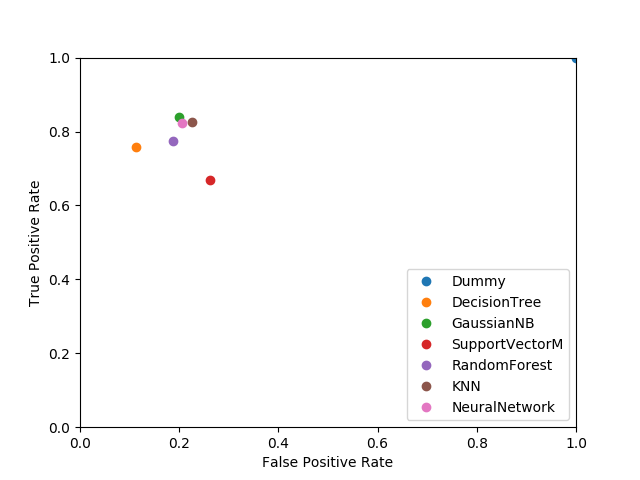
\includegraphics[width=85mm]{figures/visualizacion/roc2}
  }
  \subfigure[Preprocesado 3: Características]{
    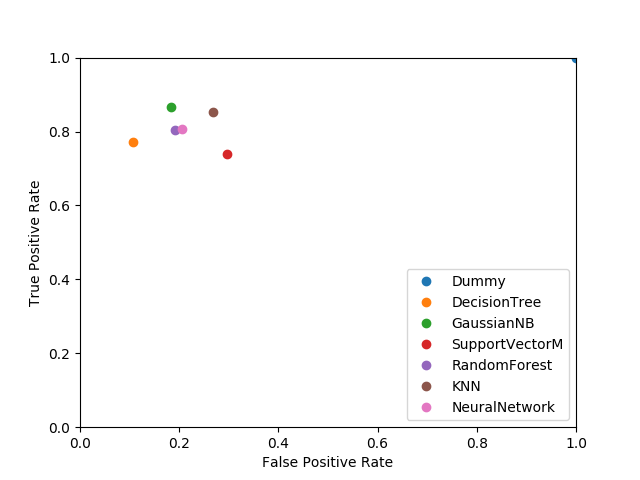
\includegraphics[width=85mm]{figures/visualizacion/roc3}
  }
  \subfigure[Preprocesado 4: Binarización]{
    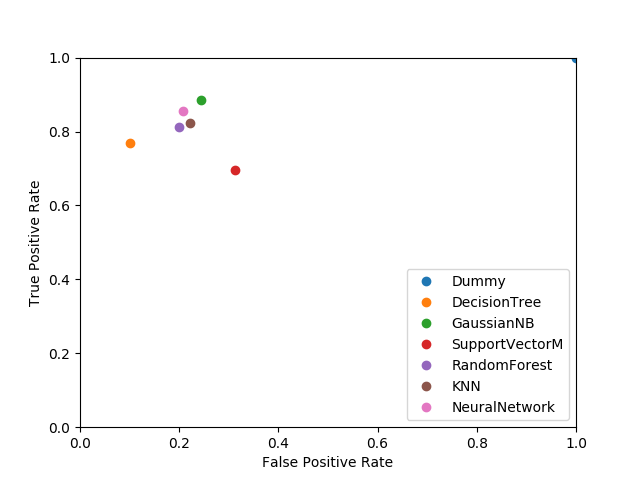
\includegraphics[width=85mm]{figures/visualizacion/roc4}
  }
  \subfigure[Preprocesado 5: Estandarización]{
    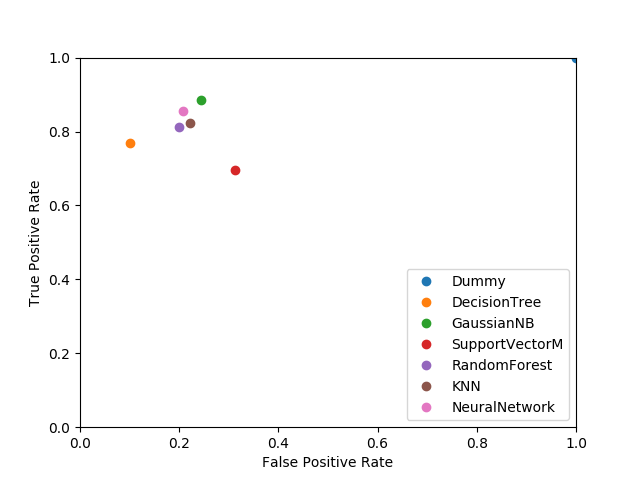
\includegraphics[width=85mm]{figures/visualizacion/roc4}
  }
  \caption{Algoritmos sobre cada preprocesado representados en el espacio ROC}
\end{figure}

\newpage

\section{Análisis de atributos}

Para cada atributo, representamos para cada posible valor el número de
instancias positivas (en azul) y negativas (en naranja). Utilizamos un
gráfico de barras apiladas, con el número de instancias malignas
abajo. En este tipo de gráficos será fácil saber cuantas instancias
malignas tienen determinado valor de una variable, y también cuantas
instancias totales. Para ver el número de instancias benignas habrá
que tener en cuenta donde empieza la barra.

\begin{figure}[H]
  \centering
  \caption{Distribución de ejemplos de cada clase para los distintos valores de BI-RADS}
  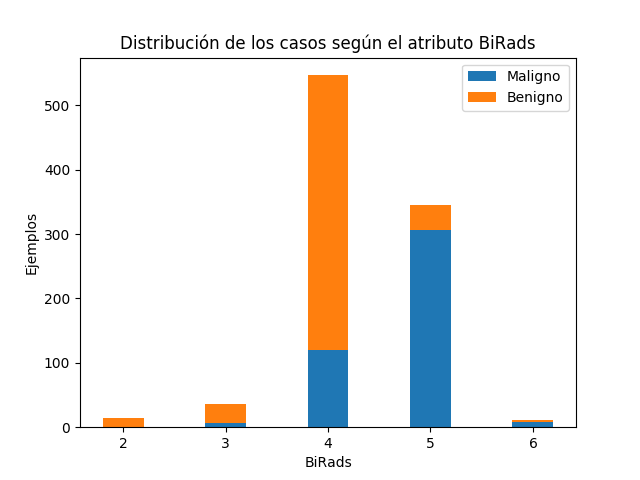
\includegraphics[width=140mm]{figures/visualizacion/birads}
  \label{fig:birads}
\end{figure}

La mayoría de instancias tienen los valores 4 y 5. Al aumentar el
valor de la variable, aumenta considerablemente la proporción de
ejemplos malignos con ese valor. Por tanto, vemos que esta variable
está altamente relacionada con la severidad del tumor.

\begin{figure}[H]
  \centering
  \caption{Distribución de ejemplos de cada clase para los distintos valores de Age}
  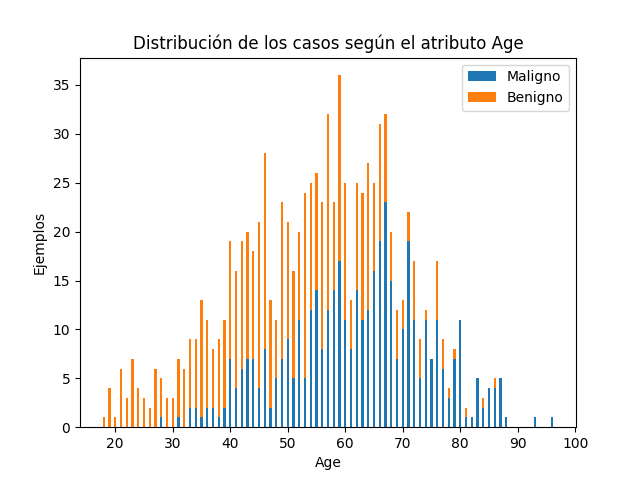
\includegraphics[width=120mm]{figures/visualizacion/age}
  \label{fig:age}
\end{figure}

Al haber tantos valores es lógico que halla impurezas, pero al igual
que antes, observamos un aumento en la proporción de ejemplos malignos
para valores altos de la variable. Por lo que también concluimos que
la edad está bastante relacionada con la severidad.

\begin{figure}[H]
  \centering
  \caption{Distribución de ejemplos de cada clase para los distintos valores de Density}
  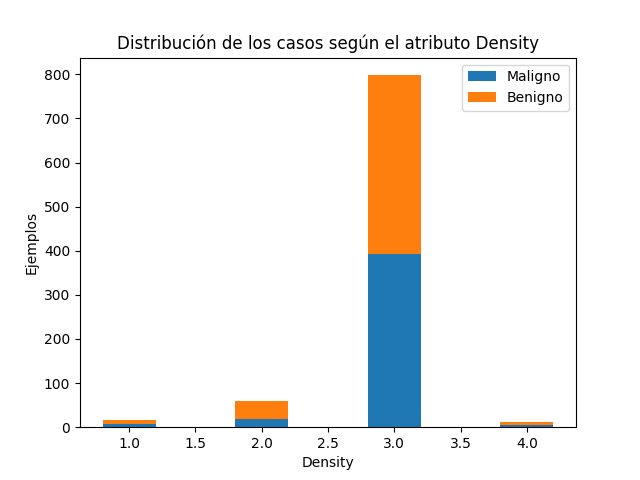
\includegraphics[width=120mm]{figures/visualizacion/density}
  \label{fig:density}
\end{figure}

Observamos que la mayoría de las instancias presentan el valor 3 de
esta variable. Además, para cada valor el número de instancias
positivas y negativas que lo presentan es prácticamente el mismo. Por
tanto, no parece que esta variable influya en la severidad del tumor.

\begin{figure}[H]
  \centering
  \caption{Distribución de ejemplos de cada clase para los distintos valores de Margin}
  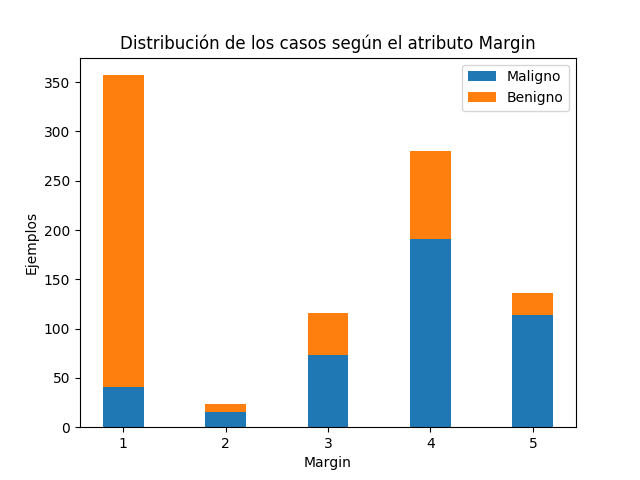
\includegraphics[width=115mm]{figures/visualizacion/margin}
  \label{fig:margin}
\end{figure}

La mayoría de las instancias que presentan el valor 1 corresponden a
tumores benignos y la mayortía de las que presentan el valor 5, a
malignos. Para el resto de valores (2, 3 y 4), la proporción de
instancias malignas es mayor que la de benignas. Concluimos que este
atributo sí puede aportarnos información sobre la severidad del tumor.

\begin{figure}[H]
  \centering
  \caption{Distribución de ejemplos de cada clase para los distintos valores de Shape}
  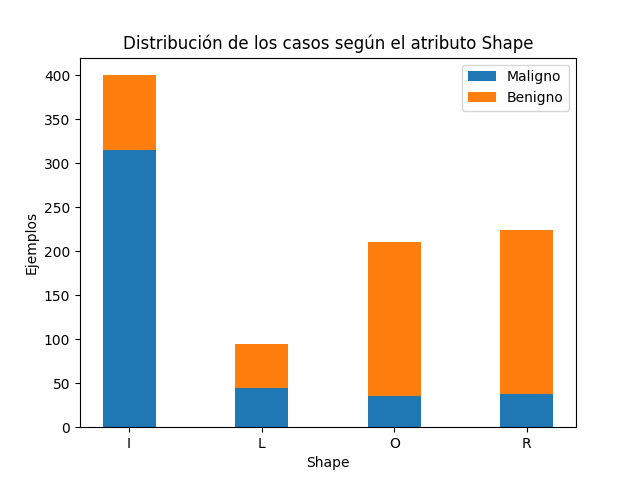
\includegraphics[width=115mm]{figures/visualizacion/shape}
  \label{fig:shape}
\end{figure}

La mayoría de instancias que presentan el valor I de esta variable,
corresponden a tumores malignos. La mayoría de las instancias que
presentan los valores O o R de esta variable, corresponden a
benignos. Mientras que hay aproximadamente las mismas instancias
benignas que malignas entre las que tienen valor L. Por tanto, esta
variable también está relacionada con la severidad.

\end{document}
